\chapter{Marco Teórico}

% En este capítulo, se presenta las principales tecnologías de detección en primer  plano del objeto en movimiento, descripción y extracción de características,  clasificación y reconocimiento del movimiento humano. Basado en el flujo óptico para la detección de objetos en movimiento. Como también la imagen de flujo de energía óptico para la detección de características de movimiento y se adoptaron redes neuronales convolucionales de región para elegir  características y reducir la dimensión. Luego, gracias al clasificador de máquina de vectores de soporte que puede ser entrenado y utilizado para clasificar y reconocer acciones; es posible distinguir efectivamente las acciones humanas y mejorar significativamente la precision del reconocimineto de las acciones humanas.

\section{Sistema de video vigilancia}
La videovigilancia consiste en la instalción de cámaras de vídeo que sirven como grabadoras las cuales guardan su contenido en un almacén digital el cual puede ser visto en un monitor central. Un sistema de video vigilancia es una instalación de seguridad cuya finalidad es el control y supervisión visual en tiempo real de instalaciones locales y remotas, mediante el uso de múltiples cámaras de vigilancia, así como de sistemas de visualización, grabación y archivo. Estos sistemas ayudan a proteger a las personas, bienes y recursos, mantienen la alerta y poseen un gran efecto disuasorio \cite{wikipedia:vvigilancia}.\\

Estos sistemas capturan imágenes y vídeos, que pueden ser comprimidos, almacenados, o enviados por una red de comunicación y pueden ser instalados en cualquier ambiente. En la figura \ref{fig:sistema_video_vigilancia} se visualiza la composición de un sistema de video vigilancia actual. Este sistema compone de un conjunto de cámaras que estan conectados directamente a un (NVR - Network Video Recorder) grabador de video en red, el cual permite la visualización de lo que las cámaras estan captando en un monitor local y por medio de una conección a un punto de acceso a internet, permite la visualización de esta transmisión en dispositivos externos a la red local\\.

\begin{figure}[H]
    \begin{center}
        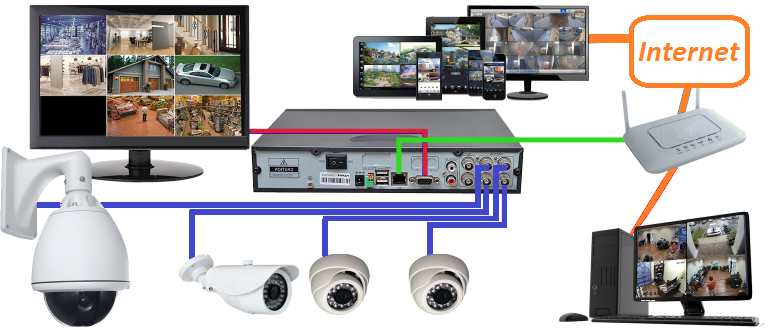
\includegraphics[width=9cm]{img/capitulo_2/sis_videovigilancia.png}
    \end{center}
    \caption{Sistema actual de videovigilancia\\Fuente: Web}
    \label{fig:sistema_video_vigilancia}
\end{figure}

La creciente demanda en el mercado de la vigilancia ha reducido costos en este tipo de sistemas, lo cual permitió que desarrolladores y fabricantes diseñen nuevas implementaciones de sistemas de video vigilancia agregándoles diversas capacidades dependiendo de la tecnología utilizada en su desarrollo. En la figura \ref{fig:surveillance-market} se muestra como el mercado global de la video vigilacia fue avaluado en 42.9 billones de dólares en 2019 y esta proyectado alcanzar a los 69.1 billones billones de dólares hasta el 2026, registrando una taza de crecimiento anual compuesta del 10\% desde el 2020 al 2026. \cite{marketsandmarkets:market-surveillance}\\

\begin{figure}[H]
    \begin{center}
        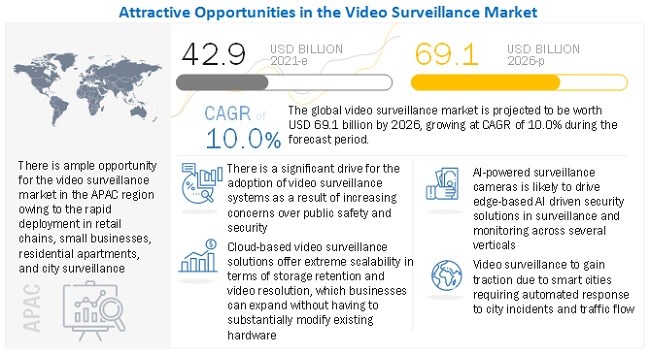
\includegraphics[width=13cm]{img/capitulo_2/surveillance-market.jpg}
    \end{center}
    \caption{Proyección del mercado de la videovigilancia\\Fuente: MarketsAndMarkets(web)}
    \label{fig:surveillance-market}
\end{figure}

El aspecto más importante a resaltar en el mercado de la videovigilancia es la potenciación de funcionalidades de estos sistemas gracias a la Inteligencia Artificial y la escalabilidad por servicios basados en la nube.Las técnicas de la inteligencia de artificial que potencian las utilidades de la videovigilancia son: vision por computadora, redes neuronales convolucionales. Machine Learning Deep Learning, reconocimiento de patrones. (A completar)\\

Para el desarrollo del prototipo propuesto se desarrolla todos los componentes involucrados en el sistema de videovigilancia como ser:
\begin{itemize}
    \item Cámaras (Nodos)
    \item Servidor TCP
    \item Servidor Web
    \item Aplicación Movil (Cliente)
\end{itemize}

A continuación se detalla los componentes que forman parte del prototipo del sistema de video vigilancia inteligente propuesto.

\section{Python}

\section{Visión por Computadora}

\section{Inteligencia Artificial}

\subsection{Redes Neuronales}

\section{Protocolos de red}

\subsection{TCP/IP}

\subsection{HTTP}

\section{Video Streaming}

\subsection{Formatos}

\subsubsection{HLS}

\subsubsection{DASH}

\section{Aplicaciones Móviles}

\subsection{Android}

\subsection{Firebase}

\subsection{Exoplayer}

\section{Metodología de desarrollo Cascada}